% Options for packages loaded elsewhere
\PassOptionsToPackage{unicode}{hyperref}
\PassOptionsToPackage{hyphens}{url}
%
\documentclass[
]{article}
\usepackage{amsmath,amssymb}
\usepackage{lmodern}
\usepackage{iftex}
\ifPDFTeX
  \usepackage[T1]{fontenc}
  \usepackage[utf8]{inputenc}
  \usepackage{textcomp} % provide euro and other symbols
\else % if luatex or xetex
  \usepackage{unicode-math}
  \defaultfontfeatures{Scale=MatchLowercase}
  \defaultfontfeatures[\rmfamily]{Ligatures=TeX,Scale=1}
\fi
% Use upquote if available, for straight quotes in verbatim environments
\IfFileExists{upquote.sty}{\usepackage{upquote}}{}
\IfFileExists{microtype.sty}{% use microtype if available
  \usepackage[]{microtype}
  \UseMicrotypeSet[protrusion]{basicmath} % disable protrusion for tt fonts
}{}
\makeatletter
\@ifundefined{KOMAClassName}{% if non-KOMA class
  \IfFileExists{parskip.sty}{%
    \usepackage{parskip}
  }{% else
    \setlength{\parindent}{0pt}
    \setlength{\parskip}{6pt plus 2pt minus 1pt}}
}{% if KOMA class
  \KOMAoptions{parskip=half}}
\makeatother
\usepackage{xcolor}
\usepackage[margin=1in]{geometry}
\usepackage{graphicx}
\makeatletter
\def\maxwidth{\ifdim\Gin@nat@width>\linewidth\linewidth\else\Gin@nat@width\fi}
\def\maxheight{\ifdim\Gin@nat@height>\textheight\textheight\else\Gin@nat@height\fi}
\makeatother
% Scale images if necessary, so that they will not overflow the page
% margins by default, and it is still possible to overwrite the defaults
% using explicit options in \includegraphics[width, height, ...]{}
\setkeys{Gin}{width=\maxwidth,height=\maxheight,keepaspectratio}
% Set default figure placement to htbp
\makeatletter
\def\fps@figure{htbp}
\makeatother
\setlength{\emergencystretch}{3em} % prevent overfull lines
\providecommand{\tightlist}{%
  \setlength{\itemsep}{0pt}\setlength{\parskip}{0pt}}
\setcounter{secnumdepth}{5}
\usepackage{booktabs,longtable,dcolumn} \usepackage{multirow,array} \usepackage{wrapfig,float} \floatplacement{figure}{H}
\ifLuaTeX
  \usepackage{selnolig}  % disable illegal ligatures
\fi
\IfFileExists{bookmark.sty}{\usepackage{bookmark}}{\usepackage{hyperref}}
\IfFileExists{xurl.sty}{\usepackage{xurl}}{} % add URL line breaks if available
\urlstyle{same} % disable monospaced font for URLs
\hypersetup{
  pdftitle={Other Metrics: QuickPay (2009-2012)},
  hidelinks,
  pdfcreator={LaTeX via pandoc}}

\title{Other Metrics: QuickPay (2009-2012)}
\author{}
\date{\vspace{-2.5em}Nov 22, 2022}

\begin{document}
\maketitle

\hypertarget{relative-delays-over-time}{%
\section{Relative delays over time}\label{relative-delays-over-time}}

\begin{itemize}
\tightlist
\item
  Sample restricted to projects for which start dates matches the one in
  API

  \begin{itemize}
  \tightlist
  \item
    This is done by using first reported ``action\_date'' and
    ``date\_signed''
  \end{itemize}
\item
  \(RelativeDelay_{it} = RelativeDelay_{it}/IntialDuration_i\)
\end{itemize}

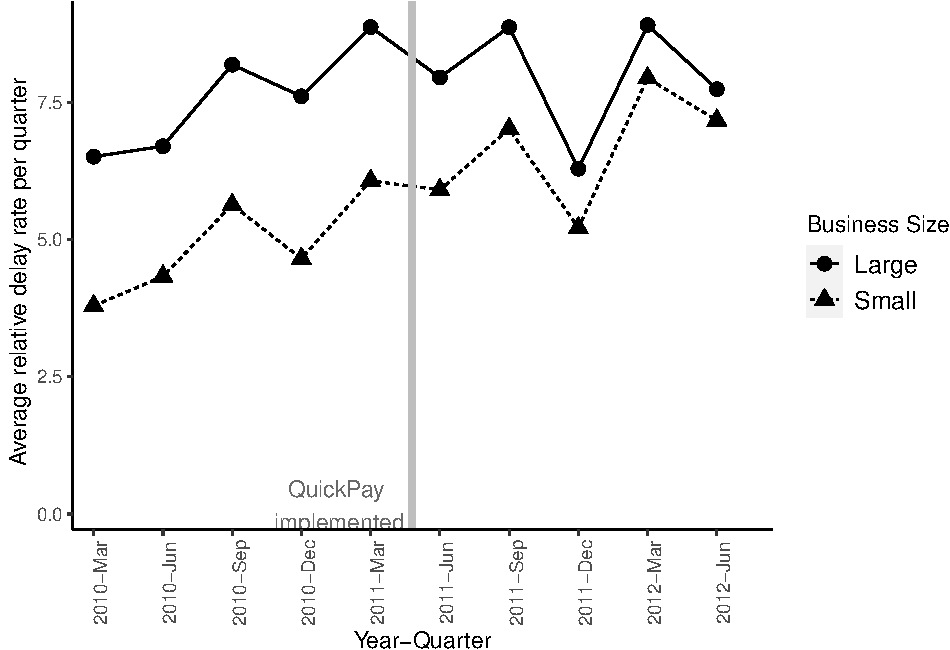
\includegraphics{qp_first_relative_delay_files/figure-latex/plot_relative_delay-1.pdf}
\#\# Normalized delay

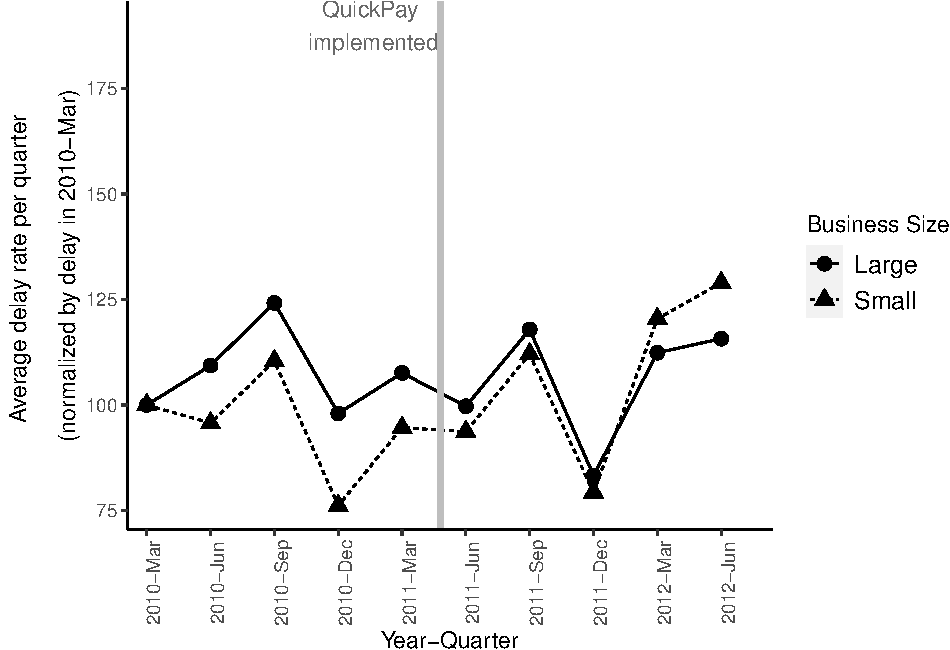
\includegraphics{qp_first_relative_delay_files/figure-latex/normalized_plot-1.pdf}

\hypertarget{baseline-regressions}{%
\section{Baseline Regressions}\label{baseline-regressions}}

\[ RelativeDelay_{it} = \beta_0 + \beta_1 Treat_i + \beta_2 Post_t + \beta_3 (Treat_i \times Post_t) + e_{it}\]

\[ \begin{aligned} RelativeDelay_{it} &=& \alpha+\beta_0 Treat_i + \beta_1 Post_t + \beta_2 (Treat_i \times Post_t)\\
&+&  X_i + (Post_t \times X_i) + \mu_t + \theta_{firm} + \lambda_{task}+ \epsilon_{it}
\end{aligned}\]

\begin{table}[H] \centering 
  \caption{Effect of QuickPay on project delay rates} 
  \label{} 
\small 
\begin{tabular}{@{\extracolsep{-2pt}}lccccc} 
\\[-1.8ex]\hline 
\hline \\[-1.8ex] 
\\[-1.8ex] & \multicolumn{5}{c}{$RelativeDelay_{it}$} \\ 
\\[-1.8ex] & (1) & (2) & (3) & (4) & (5)\\ 
\hline \\[-1.8ex] 
 $Treat_i$ & $-$1.03$^{***}$ & $-$0.82$^{***}$ & $-$0.83$^{***}$ & $-$0.44$^{***}$ & $-$0.48$^{***}$ \\ 
  & (0.11) & (0.12) & (0.12) & (0.11) & (0.11) \\ 
  & & & & & \\ 
 $Post_t$ & 0.49$^{***}$ & $-$0.83$^{***}$ &  &  &  \\ 
  & (0.11) & (0.13) &  &  &  \\ 
  & & & & & \\ 
 $Treat_i \times Post_t$ & 0.85$^{***}$ & 1.08$^{***}$ & 1.08$^{***}$ & 0.71$^{***}$ & 0.71$^{***}$ \\ 
  & (0.14) & (0.14) & (0.14) & (0.14) & (0.14) \\ 
  & & & & & \\ 
 Constant & 5.19$^{***}$ & 3.69$^{***}$ &  &  &  \\ 
  & (0.09) & (0.11) &  &  &  \\ 
  & & & & & \\ 
\hline \\[-1.8ex] 
Budget, Bids & No & Yes & Yes & Yes & Yes \\ 
$Post_t \times$  (Budget, Bids) & No & Yes & Yes & Yes & Yes \\ 
Project age & No & Yes & Yes & Yes & Yes \\ 
Year-Quarter fixed effects & No & No & Yes & Yes & Yes \\ 
Task fixed effects & No & No & No & Yes & Yes \\ 
Industry fixed effects & No & No & No & No & Yes \\ 
Observations & 257,302 & 257,234 & 257,234 & 257,234 & 257,234 \\ 
R$^{2}$ & 0.001 & 0.01 & 0.01 & 0.07 & 0.07 \\ 
Adjusted R$^{2}$ & 0.001 & 0.01 & 0.01 & 0.06 & 0.06 \\ 
\hline 
\hline \\[-1.8ex] 
\textit{Note:}  & \multicolumn{5}{r}{$^{*}$p$<$0.1; $^{**}$p$<$0.05; $^{***}$p$<$0.01} \\ 
 & \multicolumn{5}{r}{Each observation is a project-quarter.} \\ 
 & \multicolumn{5}{r}{SEs are robust and clustered at the project level.} \\ 
\end{tabular} 
\end{table}

\hypertarget{one-type-contractor}{%
\subsection{One type contractor}\label{one-type-contractor}}

\begin{table}[H] \centering 
  \caption{Effect of QuickPay on project delay rates} 
  \label{} 
\small 
\begin{tabular}{@{\extracolsep{-2pt}}lccccc} 
\\[-1.8ex]\hline 
\hline \\[-1.8ex] 
\\[-1.8ex] & \multicolumn{5}{c}{$RelativeDelay_{it}$} \\ 
\\[-1.8ex] & (1) & (2) & (3) & (4) & (5)\\ 
\hline \\[-1.8ex] 
 $Treat_i$ & $-$0.58$^{***}$ & $-$0.36$^{**}$ & $-$0.39$^{**}$ & $-$0.33$^{*}$ & $-$0.44$^{**}$ \\ 
  & (0.17) & (0.17) & (0.17) & (0.17) & (0.17) \\ 
  & & & & & \\ 
 $Post_t$ & 0.01 & $-$5.01$^{***}$ &  &  &  \\ 
  & (0.15) & (0.57) &  &  &  \\ 
  & & & & & \\ 
 $Treat_i \times Post_t$ & 1.69$^{***}$ & 1.54$^{***}$ & 1.57$^{***}$ & 1.13$^{***}$ & 1.14$^{***}$ \\ 
  & (0.21) & (0.21) & (0.21) & (0.20) & (0.20) \\ 
  & & & & & \\ 
 Constant & 6.62$^{***}$ & 10.53$^{***}$ &  &  &  \\ 
  & (0.13) & (0.49) &  &  &  \\ 
  & & & & & \\ 
\hline \\[-1.8ex] 
Budget, Bids & No & Yes & Yes & Yes & Yes \\ 
$Post_t \times$  (Budget, Bids) & No & Yes & Yes & Yes & Yes \\ 
Project age & No & Yes & Yes & Yes & Yes \\ 
Year-Quarter fixed effects & No & No & Yes & Yes & Yes \\ 
Task fixed effects & No & No & No & Yes & Yes \\ 
Industry fixed effects & No & No & No & No & Yes \\ 
Observations & 175,716 & 175,648 & 175,648 & 175,648 & 175,648 \\ 
R$^{2}$ & 0.001 & 0.05 & 0.05 & 0.10 & 0.10 \\ 
Adjusted R$^{2}$ & 0.001 & 0.05 & 0.05 & 0.09 & 0.09 \\ 
\hline 
\hline \\[-1.8ex] 
\textit{Note:}  & \multicolumn{5}{r}{$^{*}$p$<$0.1; $^{**}$p$<$0.05; $^{***}$p$<$0.01} \\ 
 & \multicolumn{5}{r}{Each observation is a project-quarter.} \\ 
 & \multicolumn{5}{r}{SEs are robust and clustered at the project level.} \\ 
\end{tabular} 
\end{table}

\hypertarget{contract-financing}{%
\section{Contract Financing}\label{contract-financing}}

\[ CF_i = \begin{cases} 1, \text{ if project } i \text{ receives contract financing}\\
0, \text{ otherwise} \end{cases}\]

\[ \begin{aligned}
RelativeDelay_{it} &=& \beta_0+\beta_1 Treat_i + \beta_2 Post_t + \beta_3 (Treat_i \times Post_t) \\
&+&\beta_4 CF_i + \beta_5 (CF_i \times Post_t) + \beta_6 (Treat_i \times Post_t \times CF_i) \\ 
&+&X_i + (Post_t \times X_i) + \mu_t + \theta_{firm} + \lambda_{task}+ \epsilon_{it}
\end{aligned}\]

\begin{table}[H] \centering 
  \caption{Financial constraints and QuickPay reform} 
  \label{} 
\small 
\begin{tabular}{@{\extracolsep{-2pt}}lccccc} 
\\[-1.8ex]\hline 
\hline \\[-1.8ex] 
\\[-1.8ex] & \multicolumn{5}{c}{$RelativeDelay_{it}$} \\ 
\\[-1.8ex] & (1) & (2) & (3) & (4) & (5)\\ 
\hline \\[-1.8ex] 
 $Treat_i$ & $-$1.00$^{***}$ & $-$0.88$^{***}$ & $-$0.88$^{***}$ & $-$0.43$^{***}$ & $-$0.47$^{***}$ \\ 
  & (0.11) & (0.12) & (0.12) & (0.11) & (0.11) \\ 
  & & & & & \\ 
 $Post_t$ & 0.37$^{***}$ & $-$0.81$^{***}$ &  &  &  \\ 
  & (0.11) & (0.13) &  &  &  \\ 
  & & & & & \\ 
 $Treat_i \times Post_t$ & 0.80$^{***}$ & 1.09$^{***}$ & 1.08$^{***}$ & 0.65$^{***}$ & 0.68$^{***}$ \\ 
  & (0.14) & (0.15) & (0.15) & (0.14) & (0.14) \\ 
  & & & & & \\ 
 $CF_i$ & 2.85$^{***}$ & 2.71$^{***}$ & 2.72$^{***}$ & $-$0.40$^{**}$ & $-$0.45$^{**}$ \\ 
  & (0.18) & (0.20) & (0.20) & (0.20) & (0.20) \\ 
  & & & & & \\ 
 $Post_t \times CF_i$ & 0.58$^{**}$ & 0.02 & 0.02 & 0.21 & 0.36 \\ 
  & (0.27) & (0.29) & (0.29) & (0.28) & (0.28) \\ 
  & & & & & \\ 
 $Post_t \times CF_i \times Treat_i$ & 0.53$^{*}$ & 0.11 & 0.16 & 0.34 & 0.12 \\ 
  & (0.30) & (0.30) & (0.30) & (0.30) & (0.30) \\ 
  & & & & & \\ 
 Constant & 4.78$^{***}$ & 3.54$^{***}$ &  &  &  \\ 
  & (0.09) & (0.10) &  &  &  \\ 
  & & & & & \\ 
\hline \\[-1.8ex] 
Budget, Bids & No & Yes & Yes & Yes & Yes \\ 
$Post_t \times $  (Budget, Bids) & No & Yes & Yes & Yes & Yes \\ 
Project age & No & Yes & Yes & Yes & Yes \\ 
Year-Quarter fixed effects & No & No & Yes & Yes & Yes \\ 
Task fixed effects & No & No & No & Yes & Yes \\ 
Industry fixed effects & No & No & No & No & Yes \\ 
Observations & 257,302 & 257,234 & 257,234 & 257,234 & 257,234 \\ 
R$^{2}$ & 0.01 & 0.01 & 0.01 & 0.07 & 0.07 \\ 
Adjusted R$^{2}$ & 0.01 & 0.01 & 0.01 & 0.06 & 0.06 \\ 
\hline 
\hline \\[-1.8ex] 
\textit{Note:}  & \multicolumn{5}{r}{$^{*}$p$<$0.1; $^{**}$p$<$0.05; $^{***}$p$<$0.01} \\ 
 & \multicolumn{5}{r}{Each observation is a project-quarter.} \\ 
 & \multicolumn{5}{r}{SEs are robust and clustered at the project level.} \\ 
\end{tabular} 
\end{table}

\hypertarget{competition}{%
\section{Competition}\label{competition}}

\hypertarget{impact-on-delays}{%
\subsection{Impact on delays}\label{impact-on-delays}}

Define
\[ SA_i = \begin{cases} 1, \text{ if project was signed after QuickPay}\\
0, \text{ otherwise} \end{cases}\]

\[ SB_i = \begin{cases} 1, \text{ if project was signed before QuickPay}\\
0, \text{ otherwise} \end{cases}\]

\hypertarget{subsample-model}{%
\subsubsection{Subsample model}\label{subsample-model}}

For a subsample of competitive or noncompetitive projects:

\[ \begin{aligned} RelativeDelay_{it} &=& \beta_0 +\beta_1 Treat_i+ \beta_2 SA_i+ \beta_3 Post_t \\&+& \beta_4 (Treat_i \times Post_t \times SA_i )+\beta_5 (Treat_i \times Post_t \times SB_i )+e_{it} \end{aligned} \]

\begin{itemize}
\item
  According to our hypothesis, \(\beta_4\) should be positive and
  significant for competitive projects, and insignificant for
  non-competitive projects.
\item
  In the following regressions, we also control for the project's age.
  Project's age is defined as the number of quarters since it first
  showed up in the sample. We include the terciles of project's age as a
  control variable.
\end{itemize}

\begin{table}[H] \centering 
  \caption{Effect of QuickPay on competitively awarded projects} 
  \label{} 
\small 
\begin{tabular}{@{\extracolsep{-2pt}}lccccc} 
\\[-1.8ex]\hline 
\hline \\[-1.8ex] 
\\[-1.8ex] & \multicolumn{5}{c}{$RelativeDelay_{it}$  } \\ 
\\[-1.8ex] & (1) & (2) & (3) & (4) & (5)\\ 
\hline \\[-1.8ex] 
 $Treat_i$ & $-$1.50$^{***}$ & $-$1.28$^{***}$ & $-$1.31$^{***}$ & $-$0.48$^{***}$ & $-$0.56$^{***}$ \\ 
  & (0.12) & (0.13) & (0.13) & (0.12) & (0.12) \\ 
  & & & & & \\ 
 $SA_i$ & $-$2.60$^{***}$ & $-$1.33$^{***}$ & $-$2.33$^{***}$ & $-$2.51$^{***}$ & $-$2.49$^{***}$ \\ 
  & (0.16) & (0.16) & (0.18) & (0.18) & (0.18) \\ 
  & & & & & \\ 
 $Post_t$ & 2.22$^{***}$ & 0.35$^{**}$ &  &  &  \\ 
  & (0.15) & (0.18) &  &  &  \\ 
  & & & & & \\ 
 $Treat_i \times SB_i \times Post_t$ & 0.28 & 0.47$^{**}$ & 0.53$^{***}$ & 0.37$^{*}$ & 0.38$^{**}$ \\ 
  & (0.19) & (0.20) & (0.20) & (0.19) & (0.19) \\ 
  & & & & & \\ 
 $Treat_i \times SA_i \times Post_t$ & 0.87$^{***}$ & 1.13$^{***}$ & 1.10$^{***}$ & 1.05$^{***}$ & 1.06$^{***}$ \\ 
  & (0.18) & (0.19) & (0.19) & (0.18) & (0.18) \\ 
  & & & & & \\ 
 Constant & 5.35$^{***}$ & 3.95$^{***}$ &  &  &  \\ 
  & (0.10) & (0.12) &  &  &  \\ 
  & & & & & \\ 
\hline \\[-1.8ex] 
Budget, Bids & No & Yes & Yes & Yes & Yes \\ 
$Post_t \times $  (Budget, Bids) & No & Yes & Yes & Yes & Yes \\ 
Project age & No & Yes & Yes & Yes & Yes \\ 
Year-Quarter fixed effects & No & No & Yes & Yes & Yes \\ 
Task fixed effects & No & No & No & Yes & Yes \\ 
Industry fixed effects & No & No & No & No & Yes \\ 
Observations & 208,724 & 208,656 & 208,656 & 208,656 & 208,656 \\ 
R$^{2}$ & 0.01 & 0.01 & 0.01 & 0.07 & 0.08 \\ 
Adjusted R$^{2}$ & 0.01 & 0.01 & 0.01 & 0.07 & 0.07 \\ 
\hline 
\hline \\[-1.8ex] 
\textit{Note:}  & \multicolumn{5}{r}{$^{*}$p$<$0.1; $^{**}$p$<$0.05; $^{***}$p$<$0.01} \\ 
 & \multicolumn{5}{r}{Each observation is a project-quarter.} \\ 
 & \multicolumn{5}{r}{SEs are robust and clustered at the project level.} \\ 
 & \multicolumn{5}{r}{Sample restricted to fully competed projects.} \\ 
\end{tabular} 
\end{table}

\begin{table}[H] \centering 
  \caption{Non-competitive projects and QuickPay law} 
  \label{} 
\small 
\begin{tabular}{@{\extracolsep{-2pt}}lcccc} 
\\[-1.8ex]\hline 
\hline \\[-1.8ex] 
\\[-1.8ex] & \multicolumn{4}{c}{$RelativeDelay_{it}$} \\ 
\\[-1.8ex] & (1) & (2) & (3) & (4)\\ 
\hline \\[-1.8ex] 
 $Treat_i$ & 1.60$^{***}$ & 1.61$^{***}$ & 1.64$^{***}$ & 0.04 \\ 
  & (0.29) & (0.29) & (0.29) & (0.31) \\ 
  & & & & \\ 
 $SA_i$ & $-$0.92$^{***}$ & 0.19 & 0.03 & $-$0.47$^{*}$ \\ 
  & (0.22) & (0.23) & (0.29) & (0.28) \\ 
  & & & & \\ 
 $Post_t$ & $-$0.07 & $-$1.37$^{***}$ &  &  \\ 
  & (0.23) & (0.39) &  &  \\ 
  & & & & \\ 
 $Treat_i \times SB_i \times Post_t$ & 2.43$^{***}$ & 2.30$^{***}$ & 2.27$^{***}$ & 1.93$^{***}$ \\ 
  & (0.42) & (0.42) & (0.42) & (0.42) \\ 
  & & & & \\ 
 $Treat_i \times SA_i \times Post_t$ & 0.42 & 0.28 & 0.32 & $-$0.07 \\ 
  & (0.41) & (0.41) & (0.41) & (0.40) \\ 
  & & & & \\ 
 Constant & 4.58$^{***}$ & 3.62$^{***}$ &  &  \\ 
  & (0.18) & (0.36) &  &  \\ 
  & & & & \\ 
\hline \\[-1.8ex] 
Budget, Bids & No & Yes & Yes & Yes \\ 
$Post_t \times $  (Budget, Bids) & No & Yes & Yes & Yes \\ 
Project age & No & Yes & Yes & Yes \\ 
Year-Quarter fixed effects & No & No & Yes & Yes \\ 
Task fixed effects & No & No & No & Yes \\ 
Observations & 48,578 & 48,578 & 48,578 & 48,578 \\ 
R$^{2}$ & 0.01 & 0.01 & 0.02 & 0.08 \\ 
Adjusted R$^{2}$ & 0.01 & 0.01 & 0.01 & 0.07 \\ 
\hline 
\hline \\[-1.8ex] 
\textit{Note:}  & \multicolumn{4}{r}{$^{*}$p$<$0.1; $^{**}$p$<$0.05; $^{***}$p$<$0.01} \\ 
 & \multicolumn{4}{r}{Each observation is a project-quarter.} \\ 
 & \multicolumn{4}{r}{SEs are robust and clustered at the project level.} \\ 
 & \multicolumn{4}{r}{Sample restricted to non-competed projects.} \\ 
\end{tabular} 
\end{table}

\hypertarget{four-way-interaction}{%
\subsubsection{Four-way interaction}\label{four-way-interaction}}

We run the following model:

\[\begin{aligned} RelativeDelay_{it} &=& \beta_0 +\beta_1 Treat_i+ \beta_2 StartedAfterQP_i+ \beta_3 Post_t+ \beta_4 Competitive_i\\ && +  \beta_5 (Treat_i \times Competitive_i) + \beta_6 (Post_t \times Competitive_i)\\ && +  \beta_7 (StartedAfterQP_i \times Competitive_i) +\beta_8 (Treat_i \times Post_t)\\ && + \beta_9 (Treat_i \times Post_t \times Competitive_i) \\ && + \beta_{10} (Treat_i \times Post_t \times StartedAfterQP_i )\\ && + \beta_{11} (Treat_i \times Post_t \times StartedAfterQP_i \times Competitive_i) + e_{it} \end{aligned}\]

\textbf{Interpretation:}

\begin{itemize}
\tightlist
\item
  \(\beta_9\) is the difference between treatment effect for competitive
  and non-competitive projects signed before quickpay.
\item
  \(\beta_9 + \beta_{11}\) is the difference between treatment effect
  for competitive and non-competitive projects signed \emph{after}
  quickpay.
\item
  \(\beta_{11}\) is our coefficient of interest because it tells us how
  much of the difference is there due to ``aggressive bidding'' after
  the policy.
\end{itemize}

\begin{table}[H] \centering 
  \caption{Effect of Competition After QuickPay: Quickpay 2009-2011} 
  \label{} 
\small 
\begin{tabular}{@{\extracolsep{-3pt}}lcccccc} 
\\[-1.8ex]\hline 
\hline \\[-1.8ex] 
\\[-1.8ex] & \multicolumn{6}{c}{$RelativeDelay_{it}$  } \\ 
\\[-1.8ex] & (1) & (2) & (3) & (4) & (5) & (6)\\ 
\hline \\[-1.8ex] 
 $Treat_i$ & 1.60$^{***}$ & 1.59$^{***}$ & 1.61$^{***}$ & 1.64$^{***}$ & 0.19 & 0.17 \\ 
  & (0.29) & (0.29) & (0.29) & (0.29) & (0.29) & (0.29) \\ 
  & & & & & & \\ 
 $StartedAfterQP_i$ & $-$0.92$^{***}$ & $-$0.75$^{***}$ & 0.22 & $-$0.63$^{***}$ & $-$1.09$^{***}$ & $-$1.08$^{***}$ \\ 
  & (0.22) & (0.22) & (0.22) & (0.24) & (0.23) & (0.23) \\ 
  & & & & & & \\ 
 $Competitive_i$ & 0.77$^{***}$ & 0.69$^{***}$ & 0.79$^{***}$ & 0.82$^{***}$ & $-$0.48$^{**}$ & $-$0.35$^{*}$ \\ 
  & (0.21) & (0.21) & (0.21) & (0.21) & (0.21) & (0.21) \\ 
  & & & & & & \\ 
 $Post_t$ & $-$0.07 & $-$0.57$^{**}$ & $-$1.52$^{***}$ &  &  &  \\ 
  & (0.23) & (0.23) & (0.24) &  &  &  \\ 
  & & & & & & \\ 
 $Treat_i \times Competitive_i$ & $-$3.10$^{***}$ & $-$2.97$^{***}$ & $-$2.89$^{***}$ & $-$2.95$^{***}$ & $-$0.72$^{**}$ & $-$0.76$^{**}$ \\ 
  & (0.31) & (0.32) & (0.32) & (0.32) & (0.32) & (0.32) \\ 
  & & & & & & \\ 
 $Post_t \times Competitive_i$ & 2.29$^{***}$ & 1.88$^{***}$ & 1.84$^{***}$ & 1.88$^{***}$ & 0.96$^{***}$ & 0.89$^{***}$ \\ 
  & (0.27) & (0.28) & (0.28) & (0.28) & (0.27) & (0.27) \\ 
  & & & & & & \\ 
 $StartedAfterQP_i \times Competitive_i$ & $-$1.68$^{***}$ & $-$1.56$^{***}$ & $-$1.55$^{***}$ & $-$1.52$^{***}$ & $-$1.28$^{***}$ & $-$1.28$^{***}$ \\ 
  & (0.28) & (0.27) & (0.27) & (0.27) & (0.27) & (0.27) \\ 
  & & & & & & \\ 
 $Treat_i \times Post_t$ & 2.43$^{***}$ & 2.25$^{***}$ & 2.28$^{***}$ & 2.32$^{***}$ & 1.64$^{***}$ & 1.60$^{***}$ \\ 
  & (0.42) & (0.42) & (0.42) & (0.42) & (0.42) & (0.42) \\ 
  & & & & & & \\ 
 $Treat_i \times Post_t \times Competitive_i$ & $-$2.15$^{***}$ & $-$1.74$^{***}$ & $-$1.80$^{***}$ & $-$1.79$^{***}$ & $-$1.25$^{***}$ & $-$1.21$^{***}$ \\ 
  & (0.47) & (0.47) & (0.46) & (0.46) & (0.46) & (0.46) \\ 
  & & & & & & \\ 
 $Treat_i \times Post_t \times StartedAfterQP_i$ & $-$2.01$^{***}$ & $-$2.02$^{***}$ & $-$2.04$^{***}$ & $-$2.01$^{***}$ & $-$1.80$^{***}$ & $-$1.87$^{***}$ \\ 
  & (0.44) & (0.43) & (0.43) & (0.43) & (0.43) & (0.43) \\ 
  & & & & & & \\ 
 $Treat_i \times Post_t \times StartedAfterQP_i \times Competitive_i$ & 2.60$^{***}$ & 2.63$^{***}$ & 2.70$^{***}$ & 2.60$^{***}$ & 2.49$^{***}$ & 2.58$^{***}$ \\ 
  & (0.48) & (0.48) & (0.48) & (0.48) & (0.47) & (0.47) \\ 
  & & & & & & \\ 
 Constant & 4.58$^{***}$ & 4.37$^{***}$ & 3.18$^{***}$ &  &  &  \\ 
  & (0.18) & (0.18) & (0.18) &  &  &  \\ 
  & & & & & & \\ 
\hline \\[-1.8ex] 
Budget, Bids & No & Yes & Yes & Yes & Yes & Yes \\ 
$Post_t \times $  (Budget, Bids) & No & Yes & Yes & Yes & Yes & Yes \\ 
Project age & No & No & Yes & Yes & Yes & Yes \\ 
Year-Quarter fixed effects & No & No & No & Yes & Yes & Yes \\ 
Task fixed effects & No & No & No & No & Yes & Yes \\ 
Industry fixed effects & No & No & No & No & No & Yes \\ 
Observations & 257,302 & 257,234 & 257,234 & 257,234 & 257,234 & 257,234 \\ 
R$^{2}$ & 0.01 & 0.01 & 0.01 & 0.01 & 0.07 & 0.07 \\ 
Adjusted R$^{2}$ & 0.01 & 0.01 & 0.01 & 0.01 & 0.06 & 0.06 \\ 
\hline 
\hline \\[-1.8ex] 
\textit{Note:}  & \multicolumn{6}{r}{$^{*}$p$<$0.1; $^{**}$p$<$0.05; $^{***}$p$<$0.01} \\ 
 & \multicolumn{6}{r}{Each observation is a project-quarter.} \\ 
 & \multicolumn{6}{r}{SEs are robust and clustered at the project level.} \\ 
\end{tabular} 
\end{table}

\end{document}
